\chapter{Capítulo 3}

Este capítulo cobre toda os conceitos fundamentais e teorias necessárias para compreender o projeto apresentando nesse documento.

\section{Processos de ETL}

O ETL é uma sigla para o processo de Extração, Transformação e Carregamento (do inglês extract -transform - load). Ele é uma integração de dados composta por três etapas de tratamentos de dados. Responsável por consilidar os dados em um repositório centralizado, chamado de Data Warehouse, e otimizado para análise. Podemos conferir seu processo descrito abaixo e graficamente através da Figura\ref{fig:etl_process}. \cite{ucommerce_etl}

\begin{itemize}
    \item \textbf{Extração:} Sua primeira fase se trata da coleta de dados brutos das fontes originais. A partir disso, os dados são extraídos para um único formato.
    \item \textbf{Transformação:} Em segundo lugar, a etapa de transformar envolve a limpeza dos dados. Onde os dados extraídos são tratados, padronizados e eliminam os erros e inconsistências dos arquivos originais. Assim, podendo serem analisados.
    \item \textbf{Carregamento:} Após os tratamentos dos dados, podemos partir para o carregamento. Nessa fase, os dados são transmitidos realizando a carga de dados no Data Warehouse.
\end{itemize}

\begin{figure}[H]
  \centering
  \caption{Processo de ETL}\label{fig:etl_process}
  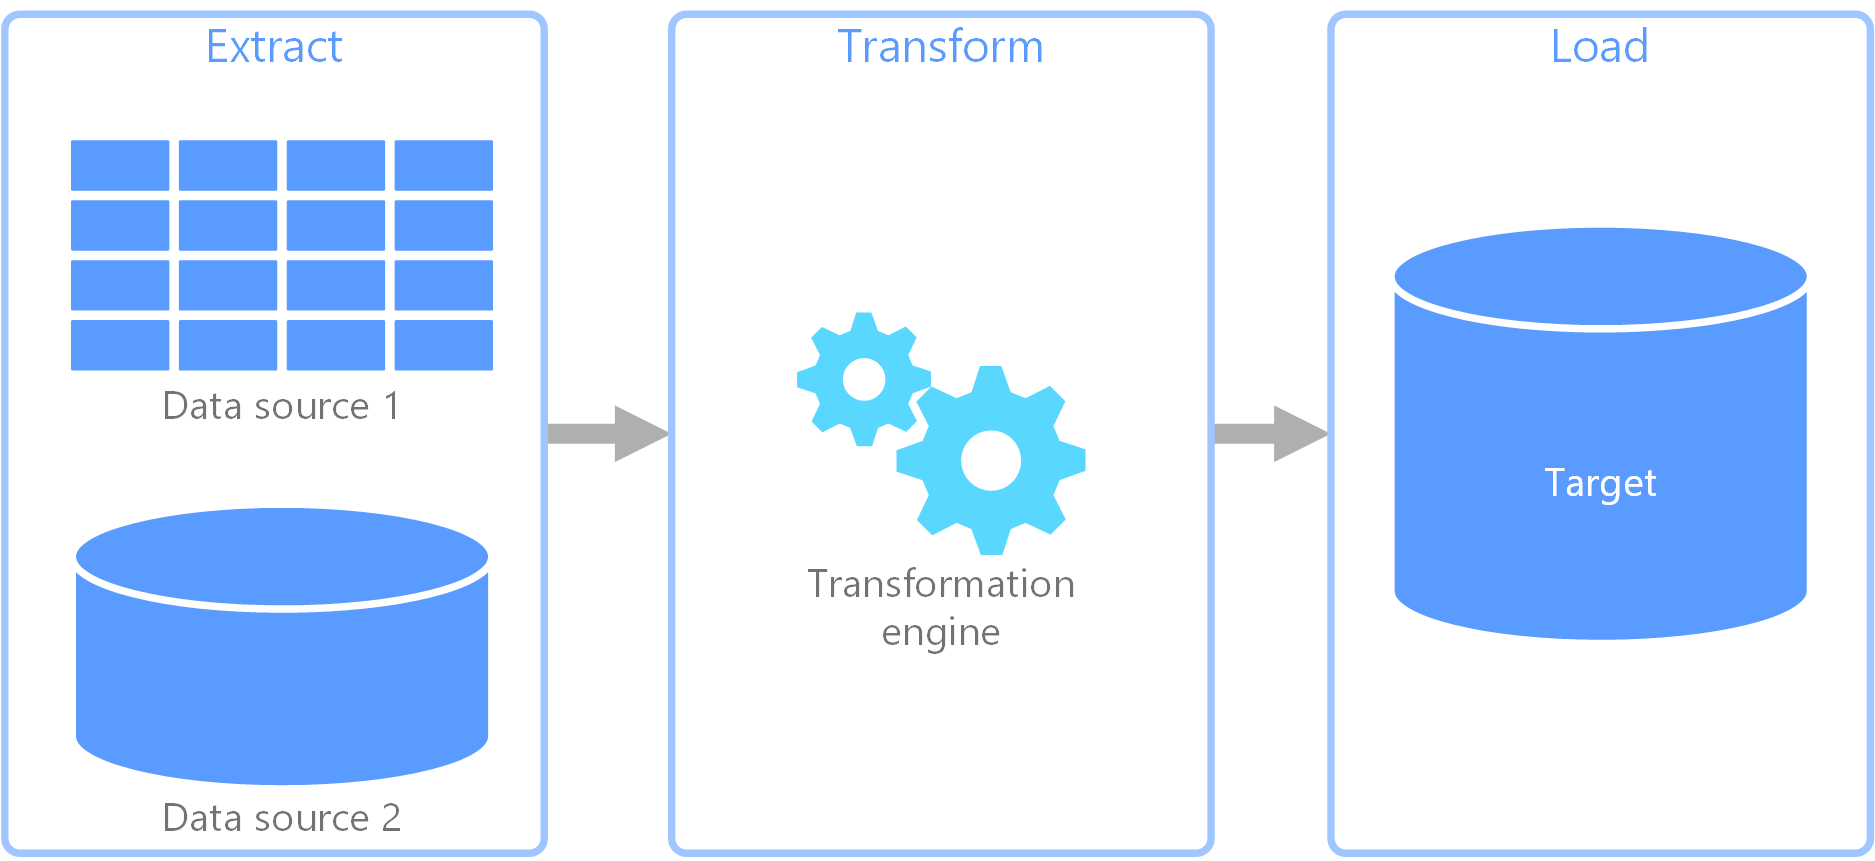
\includegraphics[width=.6\linewidth]{imagens/etl.png}
  \par
  \footnotesize{Fonte:\cite{microsoft_etl}.}
\end{figure}

\subsection{Data Warehouse}

Um data warehouse se trata de um repositório centralizado que contenha todos dados atualizados e necessários para uma organização.

Os dados são importados de diversos tipos de fontes e servem para agregar dados brutos (desestruturados) tanto quanto dados processados (estruturados) através do processo de ETL.\cite{talent500_dwdm}

Analistas de negócios, engenheiros de dados, cientistas de dados e tomadores de decisões acessam os dados por meio de ferramentas de business intelligence (BI), clientes SQL e outras aplicações de análise.

\begin{figure}[H]
  \centering
  \caption{Arquitetura de um Data Warehouse}\label{fig:datawarehouse}
  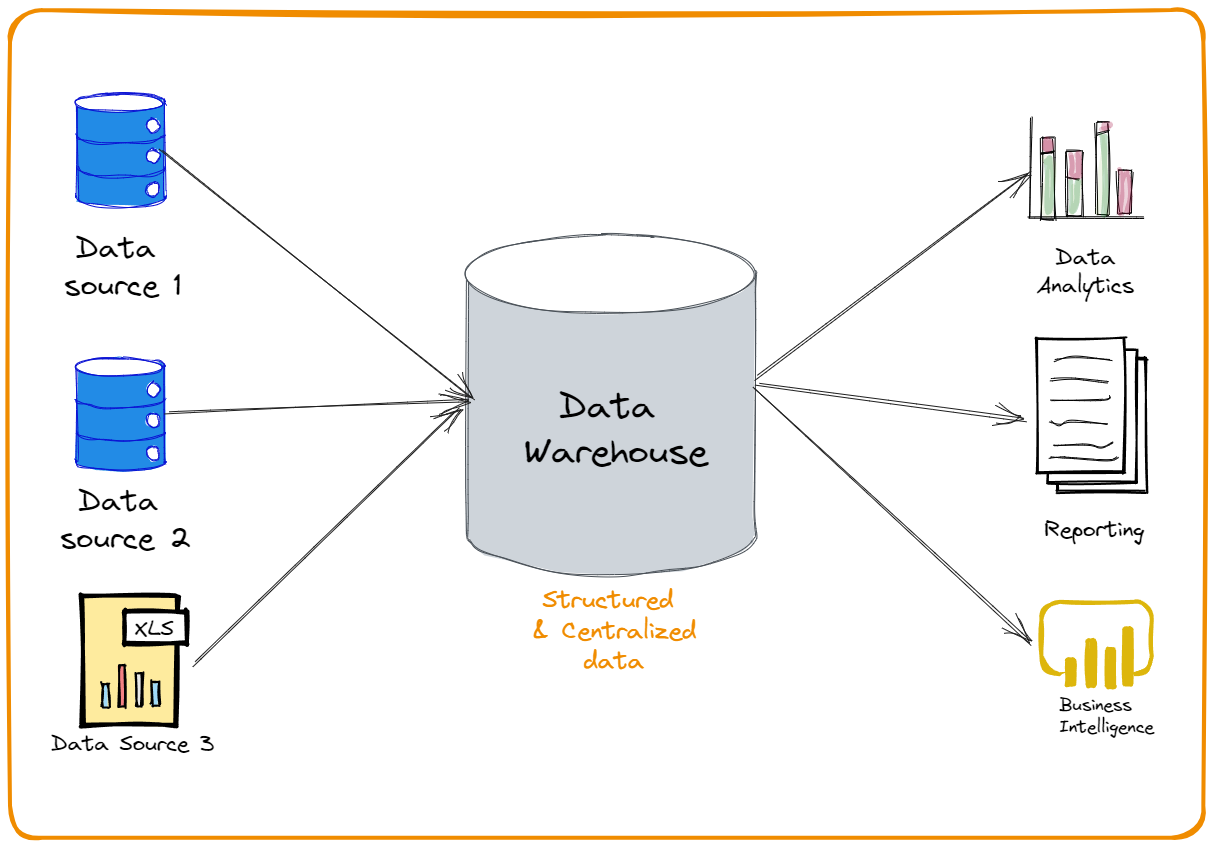
\includegraphics[width=.6\linewidth]{imagens/datawarehouse.png}
  \par
  \footnotesize{Fonte:\cite{aws_dwh}}
\end{figure}

\section{Ferramentas utilizadas para o desenvolvimento}
\subsection{Visual Studio Code}

O Visual Studio Code é um editor de código-fonte leve, mas poderoso, que é executado na área de trabalho e está disponível para Windows, macOS e Linux. Ele vem com suporte integrado para JavaScript, TypeScript e Node.js, além de um rico ecossistema de extensões para outras linguagens e ambientes de execução (como C++, C\#, Java, Python, PHP, Go, .NET).\cite{microsoft_vs}

Além disso, é possível integrar a IDE com ferramentas como debuugers, IAs e verisonamento de controle de código, aumentando a produtividade do processo de desenvolvimento.

\subsection{Python}

Python é uma linguagem de alto nivel versátil, comumente usando no contexto da engenharia de dados. Posusi uma sintaxe simples e legível, tornando acessível para iniciantes e poderosa para usuários avançados. A linguagem oferece um grande ecossistema de librarys (pacotes), como DuckDB, azure-storage-blob, PyYAML, entre outros, essenciais para o projeto. Esses pacotes provém robustez para manipulação de dados, a base do trabalho que está sendo tratado. Além disso, a facilidade da integração de outros tipos de arquivos, como JSON, YML, CSV, Excel e bancos de dados é um diferencial da linguagem. Diante dessas características, Python foi a melhor escolha para atuar como orquestrador central do pipeline de ETL.\cite{python_about}

\subsection{Package: azure-storage-blob}

O Armazenamento de Blobs do Azure é a solução de armazenamento de objetos da Microsoft para a nuvem. O armazenamento de blobs é otimizado para armazenar quantidades massivas de dados não estruturados, como dados de texto ou binários.

O armazenamento de blobs é ideal para armazenar arquivos para acesso distribuído, dados para backup e restauração, recuperação de desastres. arquivamento, dados para análise por um serviço local ou hospedado no Azure.\cite{pypi_azureblob}

\subsection{Package: requests}

requests permite o envio de requisições HTTP de forma extremamente fácil. Ela abstrai a complexidade das operações e facilita o envio de requisições como GET, POST e outras requisições. Utilizado para interagir com interfaces RESTful API e serviços web em sistemas de back-end.\cite{requests_docs}

\subsection{Package: PyYAML}

YAML é um formato de serialização de dados projetado para legibilidade humana e interação com linguagens de script. O PyYAML é um analisador (parser) e emissor de YAML para Python.

O PyYAML apresenta um analisador completo para YAML 1.1, suporte a Unicode, suporte a pickle, uma API de extensão capaz e mensagens de erro compreensíveis. O PyYAML suporta as tags padrão do YAML e fornece tags específicas do Python que permitem representar um objeto Python arbitrário.

O PyYAML é aplicável a uma ampla gama de tarefas, desde arquivos de configuração complexos até a serialização e persistência de objetos.\cite{pypi_pyyaml}

\subsection{Package: python-dotenv}

python-dotenv é uma biblioteca para ler variáveis de ambiente de um arquivo .env. Este arquivo, é utilizado para guardar chaves secretas, permitindo segurança ao projeto. Assim como credenciais de chaves de API separadas do código principal. É comumente usado em ambientes de desenvolvimento e teste.\cite{dotenv_docs}

\subsection{DuckDB}
DuckDB é um banco de dados analítico em memória, projetado para ser rápido, portátil e fácil de usar. Diferente de bancos de dados tradicionais que exigem um servidor, ele pode ser executado dentro de outros processos, o que o torna ideal para aplicações de análise de dados. Ele é facil de usar, e não necessita de dependência externas, permitindo instalação e uso em segundos. Funciona nos principais sistemas originais e possui APIs para linguagem de programações populares, incluindo \textit{Python}. Suporta a leitura direta de diferentes foramtos de arquivos, como CSV, Parquet e JSON, podendo se conectar em armazenamentos de núvem. Além  de tudo, é muito rápido, executando consultas analíticas em alta velocidade, utilizando processamento paralelo para lidar com grandes volumes de dados.\cite{duckdb_docs}

\subsection{JSON}

O JSON (JavaScript Object Notation) é uma ferramente leve do formato de intercâmbio eletrônico de dados. É fácil para humanos ler e escrever. E também é fácil para as máquinas transformarem e gerarem os dados. Baseado na linguagem de programação \textit{JavaScript Porgramming Language Standard ECMA-262 3rd Edition - December 1999}. É um formato completamente independente de linguagem, mas usa convenções que são familiares para programadores de diversas famílias de linguages, como C, C++, C\#, Java, Python, e outras. O que torna essas propriedas um formato ideal para intercâmbio de dados.\cite{json_org}

\begin{figure}[H]
  \centering
  \caption{Exemplo de formato de JSON}\label{fig:jsonformat}
  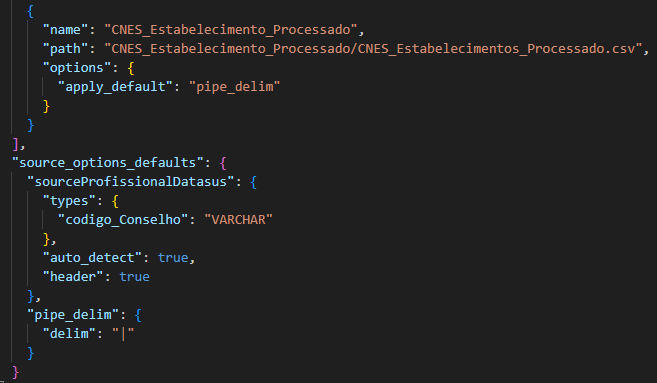
\includegraphics[width=.6\linewidth]{imagens/json.png}
  \par
  \footnotesize{Fonte: Documentos da empresa.}
\end{figure}

\subsection{Git/Github}

Git é um sistema de controle de versão distribuído que permite aos desenvolvedores rastrear mudanças no código-fonte, colaborar de forma eficiente e gerenciar o histórico do projeto com precisão. Ele suporta funcionalidades de ramificação (branching), fusão (merging) e reversão (rollback), que são essenciais para manter fluxos de trabalho de desenvolvimento limpos e organizados, especialmente em ambientes com múltiplos desenvolvedores.\cite{git_docs}

GitHub é uma plataforma de hospedagem baseada na web para controle de versão usando Git, que oferece ferramentas para rastreamento de issues, gerenciamento de projetos e automação de fluxos de trabalho através do GitHub Actions. Ele facilita a colaboração entre desenvolvedores por meio de pull requests, revisões de código e discussões, promovendo um desenvolvimento mais transparente e participativo. A utilização do GitHub é central para a gestão de código-fonte, especialmente em projetos de código aberto, simplificando os processos de integração e entrega contínua (CI/CD).\cite{github_home}

\subsection{Azure Storage Explorer}

  O Azure Storage Explorer é uma aplicação de desktop gratuita da Microsoft que fornece uma interface gráfica (GUI) para gerenciar facilmente os recursos de armazenamento do Azure. Ele funciona em Windows, macOS e Linux, permitindo que desenvolvedores, administradores de nuvem e profissionais de TI interajam com suas contas de armazenamento sem precisar escrever código ou usar linhas de comando.\cite{microsoft_azure_storage}

\subsection{R}

R é uma linguagem e um ambiente para computação estatística e gráficos. O R oferece uma ampla variedade de técnicas estatísticas (modelagem linear e não linear, testes estatísticos clássicos, análise de séries temporais, classificação, clusterização, etc.) e gráficas, e é altamente extensível. Um dos pontos fortes do R é a facilidade com que gráficos de alta qualidade, prontos para publicação, podem ser produzidos, incluindo símbolos e fórmulas matemáticas quando necessário.\cite{r_project_about}

\subsection{SQL}

A Linguagem de consulta estruturada (SQL) é uma linguagem de programação para armazenar e processar informações em um banco de dados relacional. Um banco de dados relacional armazena informações em formato tabular, com linhas e colunas representando diferentes atributos de dados e as várias relações entre os valores dos dados. Você pode usar instruções SQL para armazenar, atualizar, remover, pesquisar e recuperar informações do banco de dados. Também pode usar SQL para manter e otimizar a performance do banco de dados.\cite{aws_what_is_sql}

\subsection{YAML}

O YAML é uma linguagem legível de serialização de dados muito usada na escrita de arquivos de configuração. Dependendo, a sigla YAML pode significar em inglês "Yet Another Markup Language" (mais uma linguagem de marcação) ou "YAML Ain’t Markup Language" (YAML não é linguagem de marcação) [acrônimo recorrente]. Ambos destacam que o YAML é voltado para os dados, e não documentos. 

YAML é uma linguagem de programação famosa porque foi desenvolvida para ser fácil de ler e entender. Ele também pode ser utilizado com outras linguagens de programação.\cite{redhat_what_is_yaml}

\begin{figure}[H]
  \centering
  \caption{Exemplo de formato YAML}\label{fig:yaml}
  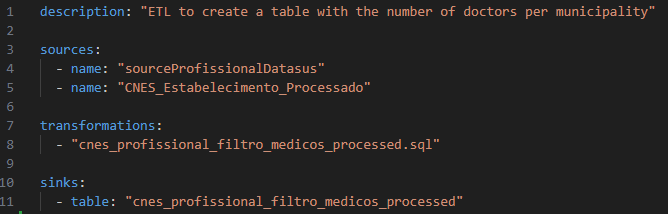
\includegraphics[width=.6\linewidth]{imagens/yaml.png}
  \par
  \footnotesize{Fonte: Documentos da empresa.}
\end{figure}

\section{Processos de ETL}